% Options for packages loaded elsewhere
\PassOptionsToPackage{unicode}{hyperref}
\PassOptionsToPackage{hyphens}{url}
\documentclass[
]{article}
\usepackage{xcolor}
\usepackage[margin=1in]{geometry}
\usepackage{amsmath,amssymb}
\setcounter{secnumdepth}{5}
\usepackage{iftex}
\ifPDFTeX
  \usepackage[T1]{fontenc}
  \usepackage[utf8]{inputenc}
  \usepackage{textcomp} % provide euro and other symbols
\else % if luatex or xetex
  \usepackage{unicode-math} % this also loads fontspec
  \defaultfontfeatures{Scale=MatchLowercase}
  \defaultfontfeatures[\rmfamily]{Ligatures=TeX,Scale=1}
\fi
\usepackage{lmodern}
\ifPDFTeX\else
  % xetex/luatex font selection
\fi
% Use upquote if available, for straight quotes in verbatim environments
\IfFileExists{upquote.sty}{\usepackage{upquote}}{}
\IfFileExists{microtype.sty}{% use microtype if available
  \usepackage[]{microtype}
  \UseMicrotypeSet[protrusion]{basicmath} % disable protrusion for tt fonts
}{}
\makeatletter
\@ifundefined{KOMAClassName}{% if non-KOMA class
  \IfFileExists{parskip.sty}{%
    \usepackage{parskip}
  }{% else
    \setlength{\parindent}{0pt}
    \setlength{\parskip}{6pt plus 2pt minus 1pt}}
}{% if KOMA class
  \KOMAoptions{parskip=half}}
\makeatother
\usepackage{longtable,booktabs,array}
\newcounter{none} % for unnumbered tables
\usepackage{calc} % for calculating minipage widths
% Correct order of tables after \paragraph or \subparagraph
\usepackage{etoolbox}
\makeatletter
\patchcmd\longtable{\par}{\if@noskipsec\mbox{}\fi\par}{}{}
\makeatother
% Allow footnotes in longtable head/foot
\IfFileExists{footnotehyper.sty}{\usepackage{footnotehyper}}{\usepackage{footnote}}
\makesavenoteenv{longtable}
\usepackage{graphicx}
\makeatletter
\newsavebox\pandoc@box
\newcommand*\pandocbounded[1]{% scales image to fit in text height/width
  \sbox\pandoc@box{#1}%
  \Gscale@div\@tempa{\textheight}{\dimexpr\ht\pandoc@box+\dp\pandoc@box\relax}%
  \Gscale@div\@tempb{\linewidth}{\wd\pandoc@box}%
  \ifdim\@tempb\p@<\@tempa\p@\let\@tempa\@tempb\fi% select the smaller of both
  \ifdim\@tempa\p@<\p@\scalebox{\@tempa}{\usebox\pandoc@box}%
  \else\usebox{\pandoc@box}%
  \fi%
}
% Set default figure placement to htbp
\def\fps@figure{htbp}
\makeatother
\setlength{\emergencystretch}{3em} % prevent overfull lines
\providecommand{\tightlist}{%
  \setlength{\itemsep}{0pt}\setlength{\parskip}{0pt}}
\usepackage{fvextra}
\DefineVerbatimEnvironment{Highlighting}{Verbatim}{breaklines,commandchars=\\\{\}}
\usepackage{indentfirst}
\setlength{\parindent}{2em}
\setlength{\parskip}{0.5em}
\usepackage{bookmark}
\IfFileExists{xurl.sty}{\usepackage{xurl}}{} % add URL line breaks if available
\urlstyle{same}
\hypersetup{
  pdftitle={Retrieval Capabilities of Legal AI Tools},
  pdfauthor={Justin Tung},
  hidelinks,
  pdfcreator={LaTeX via pandoc}}

\title{Retrieval Capabilities of Legal AI Tools}
\author{Justin Tung\footnote{Transactional Practice Innovation Lead at
  Jackson Walker LLP. The author holds a J.D. from the University of
  Texas School of law, MSLIS from the University of Illinois, and a BA
  from Boston College.}}
\date{2026}

\begin{document}
\maketitle

{
\setcounter{tocdepth}{3}
\tableofcontents
}
\section{Abstract}\label{abstract}

Legal technology vendors offer products with different capabilities. One
capability often offered is the ability to upload documents as a custom
database and query it with an AI chat functionality. This study presents
an experiment, data, and analysis of the performance of these legal AI
tools from Westlaw, Lexis, and Harvey with different kinds and sizes of
uploaded text. I create a specified set of files and seed ``clues'' that
correspond to questions I ask the legal AI tool covering a range of
retrieval and logic tasks. The legal AI's response is evaluated on the
basis of its ability to retrieve the seeded information. This analysis
and data describes the relationship between legal AI performance and
both file set sizes and corpora types, specifically retrieval capability
and accuracy. I conclude that there are correlations between file set
size and performance, and for all tested products, a correlation between
corpora and performance. This research aims to provide data and analysis
that users of legal AI tools can use to better understand these tools
and make informed decisions about use by critically assessing the legal
AI tools along the variables used in this research.

\section{Key Terms}\label{key-terms}

Legal Research, Artificial Intelligence, Emperical Data, Database
Retrieval

\section{Submissions and
Declarations}\label{submissions-and-declarations}

The author has no financial or non-financial interest in the products
evaluated, or the outcome of the evaluation.

\section{Acknowledgments}\label{acknowledgments}

This research did not receive any funding.

\section{Background and Literature
review}\label{background-and-literature-review}

Electronic document management platforms have long been part of law
practice and are an area that generative AI has and continuyes to
disrupt. A critical element of this disruption is the ability to use
legal AI tools not just to analyze documents, but to identify relevant
documents out of many. This creates a new market for legal AI tools such
as Harvey and Legora, which are not part of large pre-existing legal
databases of authorities. Traditional legal tech platforms have also
expanded to offer legal AI tools with this functionality as well.

Despite this, there is very little independent evaluation or comparison
of available legal AI tools for this specific purpose. Some of this is
due to lack of access to multiple tools with similar functionality.
Contracts with platforms also may prohibit public disclosure of analysis
or technical findings. Another factor may be the labor required to
gather data at a scale that researchers can statistically analyze.
Consequently, while a lot of great research has been and is continually
done on the research or generative abilities of legal AI tools, there is
currently very little analysis or scrutiny of the ability of these tools
to interact with user-uploaded files.

The one study that I could identify addressing a similar question is the
Vals Legal AI Report from February 27, 2025 by Vals AI.\footnote{Vals
  AI, \emph{Vals Legal AI Report} (Feb.~2025),
  https://www.vals.ai/industry-reports/vlair-2-27-25
  {[}https://perma.cc/58WN-ZS33{]}} This study covers many different
legal AI tools and types of tasks that legal AI tools may be asked to
do. Of the many tasks, Data Extraction and Document Q\&A tests are the
most similar to the focus of my study. However, this study addresses a
fundamentally different research question, specifying no more than a
single-digit number of files as a source for a legal AI's response. This
study also confined user-uploaded files to sets of no more than 29 in
any trial and only uploading documents pertaining to that specific
trial. In this study's ``Notes on study limitation'' section, the
researchers specifically acknowledge that they were limited by the
nature of the type of documents and question/answer pairs in their
experimental design. While the Vals study is useful in addressing the
use case of users uploading small and specific sets of files, it does
not examine a use case with more files of varying relevance. Given the
fact that some of these legal AI tools allow a much larger capacity than
what the Vals AI study tests, it leaves many potential use cases
unassessed.

It is into this research gap that this research steps.

\section{Methodology}\label{methodology}

All code is available at this Git Repository:
https://github.com/JayTongue/Sherlock\_HoLLMes

Generative Artificial Intelligence was not used in any step of the
experimental design, trials, evaluations, or writing of this
experimentation or report.

\subsection{Overview:}\label{overview}

This paper evaluates the capability of different legal AI products by
grading their ability to answer questions based on a standardized set of
problems seeded throughout files containing different kinds of text
(corpora). I chose products which offered the ability to upload and
query a custom set of files with a legal AI tool. The evaluated tools
for this study were Westlaw CoCounsel, Lexis Protégé, and Harvey.

I tested five different kinds of corpora: two based on real-world data
sets and three synthesized corpora. The real-world data sets were
download from open-source online repositories. Synthetized data sets
were algorithmically generated with a variety of computational means.

The Clues that formed the questions followed standardized templates,
swapping the names of individuals, topics, and other fields so that they
do not overlap and entangle, and questions always have some element of
spontaneous iteration and variability. After creating files and clues, I
injected the clues into random places in randomly selected files in a
given set.

I then uploaded the injected file set to a legal AI tool and asked it
the corresponding questions. I then evaluated the legal AI's answers and
recorded the results.

\subsubsection{Products Tested}\label{products-tested}

The products evaluated in this study were confined to those available to
the author in late 2025 and early 2026. These tools were Westlaw
CoCounsel 2.0, Lexis Protégé, and Harvey.

Westlaw CoCounsel 2.0 is a legal AI tool released by Westlaw, a legal
publisher and research platform owned by Thomson Reuters. Westlaw
released their CoCounsel AI in August of 2025.\footnote{Thomson Reuters,
  \emph{Thomson Reuters Launches CoCounsel Legal: Transforming Legal
  Work with Agentic AI and Deep Research}, \textsc{Thomson Reuters}
  (August 5, 2025)
  https://www.thomsonreuters.com/en/press-releases/2025/august/thomson-reuters-launches-cocounsel-legal-transforming-legal-work-with-agentic-ai-and-deep-research
  {[}https://perma.cc/A5S5-PZ26{]} (last visited Feb.~17, 2026).}

Lexis is also a legal publisher and research database. They are owned by
RELX, a company based in the United Kingdom\footnote{RELX, \emph{Legal},
  \textsc{RELX}, https://www.relx.com/our-business/market-segments/legal
  {[}https://perma.cc/U9QF-BAQF{]} (last visited February 17, 2026).}.
Lexis released their legal AI product, Protégé, in January 2025 for
general availability in the United States.\footnote{LexisNexis,
  \emph{LexisNexis Introduces Protégé Personalized AI Assistant with
  Agentic AI, Making it Easier to Power Complex Legal Task Completion},
  \textsc{LexisNexis} (January 27, 2025)
  https://www.lexisnexis.com/community/pressroom/b/news/posts/lexisnexis-introduces-protege-personalized-ai-assistant-with-agentic-ai-making-it-easier-to-power-complex-legal-task-completion
  {[}https://perma.cc/77K3-QDPH{]} (last visted Feb.~17, 2026).} The
evaluated version of Lexis Protégé does not have a specific version
appociated with it, and is simply branded as ``Lexis+ with Protégé''.

Westlaw and Lexis are sometimes referred to as a duopoly because of
their dominant market positions for offering databases of legal and
law-adjacent sources. While they do not face as much competition from
other companies when it comes to legal databases, the area of legal AI
is broadly contested, with many emerging players in the field. One such
company is Harvey.

Harvey was founded in 2022 as a legal tech startup. In December of 2025,
a funding round valued the company at 8 billion dollars.\footnote{Michael
  J. de la Merced, \emph{Harvey, a Maker of A.I. Legal Software, Raises
  New Funds}, \textsc{The New York Times} (Dec.~4, 2025)
  https://www.nytimes.com/2025/12/04/business/dealbook/harvey-legal-ai.html
  {[}https://perma.cc/L222-8UHG{]} (last visited Feb.~17, 2026).} Harvey
offers a variety of legal AI products such as the ability to create
custom databases, make user-defined workflows, and iteratively produce
and generate drafts of legal documents. The version of Harvey evaluated
in this study did not have a version number.

This study confines its scope to the ability to upload a custom database
and query it with a legal AI. All three of these platforms offer this
ability. Lexis and Harvey refer to these user uploaded files as a
``vaults'', whereas Westlaw simply refers to them as ``databases''. All
seem to be analogous tools by a different name.

\subsubsection{Data Sources and File
Sets}\label{data-sources-and-file-sets}

A file set refers to the files used for a single upload and a single set
of questions. Every file set is comprised of content from one of five
corpora types with a specified number of files in the set. For instance,
an Enron file set of size 25 would contain 25 files randomly selected
from the Enron dataset.

\emph{Corpus Types}

This study used five different types of corpora, meant to span a range
of possible files in a legal setting. Files from the Contracts and Enron
datasets were high in semantic content, whereas the synthetic corpora
(Markov, Random, and Zeros) were low in semantic content. This paper
uses ``semantic content'' to refer to content which conveys cognizable
information. For instance, a clause of a contract conveys information
about the agreement between the parties, whereas a string of random
characters conveys no information. Besides the Contracts and Enron
corpora which are semantically meaningful, the Markov copora mimics the
text of legal opinions while the Random corpora mimics data which may be
encrypted or corrupted, and the Zeros corpora mimics data which may be
blank, overwritten, or redacted.

I included the random and zero data sets in this study to act as
baselines to compare legal AI performance. Their complete lack of any
human-readable language except for the clues isolates the element of
pure dilution by allowing assessment of model performance without any
confounding semantic content from the underlying corpus. It is against
these that the performance of more realistic datasets such as those made
from the contracts or enron corpora are contextually evaluated.

I included the Markov corpus because of the interesting properties of
Markov text. Specifically, although Markov text is statistically valid
by definition, it is semantically meaningless. Since one of the features
of large language models is that they process and understand text, the
Markov corpus poses an interesting comparison to truly meaningful
corpora from the real world.

File sets of the ``Contracts'' filetype were filled with files randomly
selected from the Material Contracts Corpus compiled in 2025 by Stanford
Law School. This dataset is mostly comprised of contracts publicly
available in the SEC EDGAR database. It contains the text of 1,038,766
contracts as well as metadata, totalling 156.2 GB. I downloaded this
dataset from the Material Contracts Corpus website\footnote{Peter
  Adelson and Julian Nyarko, \emph{Material Contracts Corpus},
  \textsc{Stanford Law School} https://mcc.law.stanford.edu/
  {[}https://perma.cc/XC7Z-AJ7G{]} (last visited Feb.~17, 2026).},
indexed it, and randomly sampled it for the text of file sets of this
corpus type.

File sets of the ``Enron'' filetype were filled with files randomly
selected from the Enron Email Dataset V2. Although this dataset has
received a lot of analysis and scrutiny, it is quite difficult to find
the dataset in a complete, un-filtered form. The fullest dataset
available to the author was from the Internet Archive\footnote{Enron
  Corporation, \emph{Files for edrm.enron.email.data.set.v2.xml},
  \textsc{Internet Archive}
  https://archive.org/download/edrm.enron.email.data.set.v2.xml
  {[}https://perma.cc/HYM9-72YQ{]} (last visited Feb.~17, 2026).}. These
files were downloaded, extracted, and indexed. Fully extracted, this
dataset takes 258.9 GB.

A portion of this data is machine-generated text, such as email
headings, signatures, and other computationally added information
besides the message of the actual emails. Files for an Enron type file
set contain the text of files randomly selected from this dataset.

File sets of the ``Markov'' filetype contained text generated from
Markov Chains trained on the United States Reports. Markov Chains are
mathematical descriptions of the pattern of text in a training corpora.
Simplistically, they record the statistical likelihood of any current
textual state leading to a given future textual state.\footnote{See
  e.g.~Joseph Chang, \emph{Markov Chains}, (February 2, 2007)
  http://www.stat.yale.edu/\textasciitilde pollard/Courses/251.spring2013/Handouts/Chang-MarkovChains.pdf
  {[}https://perma.cc/3S23-J3A3{]} (last visited Feb.~17, 2026) (A
  chapter of an unpublished textbook manuscript).}

I downloaded the United States Reports (1754-2014) from the Caselaw
Access Project\footnote{United States Government Publishing Office,
  \emph{United States Reports (1754-2014)}, \textsc{Caselaw Access
  Project} https://case.law/caselaw/?reporter=us
  {[}https://perma.cc/5PV9-6WMT{]} (last visited Feb.~17, 2026).}. I
first normalized the text of the opinions with a normalization function
called NFKC\footnote{Ken Whistler, \emph{Unicode Normalization Forms},
  \textsc{Unicode Standard Annex \#15} (2025-07-30)
  https://www.unicode.org/reports/tr15/ {[}https://perma.cc/Q936-SMC2{]}
  (last visited Feb.~17, 2026).}. This normalization collapsed the text
of the characters into a more manageable encoding space by changing
uncommon characters into more common characters, reducing the number of
total characters into a more manageable ``canon''. This eliminated
variations in encoding that would skew the Markov chains by modeling
unintentional or unimportant distinctions between characters. For
instance, the ``fi'' ligature defined as a single Unicode character
(U+FB01) would be transformed to ``fi'' as two separate letters through
NFKC. This step is important because the Caselaw Access Project used
Optical Character Recognition (OCR) on scans of physical
reporters.\footnote{The Library Innovation Lab Team, \emph{Transitions
  for the Caselaw Access Project}, \textsc{Library Innovation Lab}
  (Mar.~26, 2024),
  https://lil.law.harvard.edu/blog/2024/03/26/transitions-for-the-caselaw-access-project/
  {[}https://perma.cc/K6PY-9FM5{]}} While OCR is very useful for
translating physical or other non-machine coded media into a
text-encoded form, it often results in recognition errors due to
imperfections in the physical source medium.

I then tokenized the text with a regular expression that split the text
into a list of continuous characters and punctuation from the block of
normalized text. I iterated through this tokenized text to construct
3rd-order, 2nd-order, and 1st-order markov chains.\footnote{E.g. given
  the text \texttt{"We\ the\ People\ of\ the..."}, an example of a
  3rd-order markov chain would be for the key:
  \texttt{(\textquotesingle{}We\textquotesingle{},\ \textquotesingle{}the\textquotesingle{},\ \textquotesingle{}People)}
  to correspond to the value:
  \texttt{\textquotesingle{}of\textquotesingle{}}. A 2nd-order markov
  chain would pair the key:
  \texttt{(\textquotesingle{}We\textquotesingle{},\ \textquotesingle{}the\textquotesingle{})}
  with the value \texttt{\textquotesingle{}People\textquotesingle{}}. A
  1st-order markov chain would pair the key:
  \texttt{(\textquotesingle{}We\textquotesingle{})} to the value
  \texttt{\textquotesingle{}the\textquotesingle{}}. Because higher
  orders consider more context when deciding the next value, they are
  generally prefered for generating more realistic text and avoiding
  inexcapable loops.} These chains then generated text from a single
randomly selected starting 3rd-order key. If a situation was not found
as the chains generated text, the 3rd-order chain rolled back to
2nd-order, then the 1st-order chain if necessary.

Files of the Markov corporus used these chains to generate text until
the text met the target file size.

File sets of the ``Random'' filetype contained the text of characters
from generated from the /dev/urandom and /dev/random files in a linux
filesystem. These two files allow users to access the computer's random
number generator, returning a random stream of bytes based on the
computer's entropy pool.\footnote{Linux Foundation, \emph{urandom(4) -
  Linux man page}, \textsc{Linux Manual}
  https://linux.die.net/man/4/urandom {[}https://perma.cc/5CS5-V7KB{]}
  (last visited Feb.~17, 2026).}

Files in the Random file sets used a stream of random bytes from these
random generators until they contained the target number of bytes. While
the initial experimental design was to generate files that spanned the
whole range of possible byte combinations for maximum randomness, this
often led to errors when trying to encode that text into some file
types, especially DOCX. This meant that the characters that caused
errors would either have to be removed individually or with a heuristic
rule.

To curtail these issues, I regularized the data as hexadecimal strings.
Although this is a limitation on the kind of characters the files could
contain, this ensured that the characters written to Random files were
in the file type's encodable space and would therefore convert into that
file type without encoding errors.

I filled files in Random file sets with these regularized random bytes
until the text met the target file size.

Files in the Zeros file sets contained literally repeated numerical
zeros (``0''). Similarly to streamed random bytes in the Random corpus,
a function streamed zeros into files until they contained the target
file size.

\emph{Distribution Analysis}

In order to mimic a realistic file size distribution for the synthetic
corpora types (Markov, Random, and Zeros), I analyzed the file size
distribution of the two publicly available datasets (Contracts and
Enron) so that the generated files could follow roughly the same
distribution. Since I was regularizing sizes of individual files along a
set distribution, I decided to use number of files in a set as a proxy
metric for overall size of information. Since both the Contracts and
Enron datasets could be fit to a lognormal distribution, I followed an
average of their distributions when creating synthetic corpora. A less
limited study could explore the effect of different types of
distributions.

After analyzing the file sizes of both the Enron and Contracts datasets,
I fit this file size data to a lognormal distribution:

\[X = e^{\mu + \sigma Z} \sim \text{LogNormal}(\mu, \sigma)\]

where \(Z \sim \mathcal{N}(0,1)\).

\textbf{Parameters:}

\begin{itemize}
\tightlist
\item
  \(\mu\) is the mean of \(\ln X\)
\item
  \(\sigma\) is the standard deviation of \(\ln X\)
\item
  \(Z \sim \mathcal{N}(0,1)\) is a standard normal random variable
\end{itemize}

The Contracts dataset contains consistent filetypes and relatively
consistent content, fitting the lognormal distribution decently.
However, the Enron database's distribution was very irregular, with
spikes corresponding to different types of files or contents. For
instance, simple emails would tend to be one size, emails with
attachments would be another size, machine log files would be another,
etc. There were also files as small as 10 bytes, which were functionally
useless for the purposes of this research. When calculating parameters
and randomly selecting files from both the Contracts and Enron datasets,
I implemented a 1KB floor to eliminate these miniscule files. I did not
implement an upper limit of file size.

{\def\LTcaptype{none} % do not increment counter
\begin{longtable}[]{@{}
  >{\raggedright\arraybackslash}p{(\linewidth - 4\tabcolsep) * \real{0.2667}}
  >{\raggedright\arraybackslash}p{(\linewidth - 4\tabcolsep) * \real{0.3667}}
  >{\raggedright\arraybackslash}p{(\linewidth - 4\tabcolsep) * \real{0.3667}}@{}}
\toprule\noalign{}
\begin{minipage}[b]{\linewidth}\raggedright
Metric
\end{minipage} & \begin{minipage}[b]{\linewidth}\raggedright
Contracts Dataset
\end{minipage} & \begin{minipage}[b]{\linewidth}\raggedright
Enron Dataset
\end{minipage} \\
\midrule\noalign{}
\endhead
\bottomrule\noalign{}
\endlastfoot
\textbf{\(\mu\) (mu)} & 10.866 & 9.0723 \\
\textbf{\(\sigma\) (sigma)} & 1.4167 & 1.8434 \\
\textbf{Median} & 52 KB & 1.2 KB \\
\textbf{95\% Range} & 2 KB, 900 KB & 10 bytes, 10 MB \\
\textbf{Notes} & Well-behaved distribution & Heavy right tail with
extreme outliers \\
\end{longtable}
}

Despite the lognormal distribution not fitting well to the Enron
dataset, the lognormal distribution was the one that fit the model the
best without breaking the distribution down into different functions or
over-fitting with a high-order polynomial. After fitting, I averaged the
Mu and Sigma parameters from both datasets to create parameter targets
for the synthetic data sets. These averaged parameters yielded file size
targets sitting in between the Contracts and Enron datasets.

\begin{itemize}
\tightlist
\item
  \(\mu = 9.96915\),
\item
  \(\sigma = 1.63005\)
\end{itemize}

I used these parameters to generate target file sizes to be filled with
Markov text, random characters, or zeros.

\paragraph{File Types}\label{file-types}

Each commercial vendor permitted different types of files. Harvey was
the most permissive, allowing PDF, DOCX, RTF, TXT, EML, MSG, XLS, XLSX,
CSV, PPT, PPTX, HTML, as well as code files written in various
programming languages.\footnote{Harvey, \emph{Vault: Analyze Large
  Document Sets at Scale}, \textsc{Harvey Support} (Feb 4, 2026)
  https://help.harvey.ai/articles/vault {[}https://perma.cc/75JL-7B7E{]}
  (last visited Feb.~17, 2026).} Westlaw allows PNG, JPEG, Word, Excel,
CVS, PDF, and zips of each of the other accepted file types.\footnote{Thomson
  Reuters, \emph{Supported file types}, \textsc{Thomson Reuters}
  https://www.thomsonreuters.com/en-us/help/cocounsel/tax-audit-accounting/conversations/supported-file-types
  {[}https://perma.cc/WN77-PBBY{]} (last visited Feb.~17, 2026).} Lexis
was the most restrictive, allowing only PDF, DOC, DOCX, TXT, and ZIP
files.\footnote{Lexis+, \emph{Upload Documents}, \textsc{LexisNexis}
  https://help.lexisnexis.com/Flare/lexisplusai/US/en\_US/Content/FAQ/upload.htm?Highlight=pdf
  {[}https://perma.cc/4MSP-CYEG{]} (last visited Feb.~17, 2026)}

Note that Lexis' restrictiveness, to some extent, is arbitrary. Many of
the other file formats such as CSV, HTML, and EML can be opened as plain
text files and do not exist in a specialized encoding that requires an
additional parser. This restrictiveness is an interesting business
and/or engineering decision, especially since documentation for other
Lexis tools seems to show that other tools had permit more file
types.\footnote{LexisNexis, \emph{File Formats and Limits},
  \textsc{LexisNexis}
  https://help.lexisnexis.com/Flare/casemaponline/US/en\_US/Content/file\_format\_limit.htm
  {[}https://perma.cc/7J4S-LW6F{]} (last visited Feb.~17, 2026)}

However, due to this restriction, I chose to randomize files as either
PDF, TXT, or DOCX in approximately equal proportion since the permitted
ZIPs would just be decompressed into those file types before actual
processing. Additionally, DOCX has largely superseded DOC as a file
type.

I converted the target text to PDF with the \texttt{reportlab} Python
library\footnote{\textsc{ReportLab Docs}, \emph{Andy Robinson} et al.,
  https://docs.reportlab.com/ (last accessed March 6, 2026).}, and
converted to DOCX with the \texttt{python-docx} library\footnote{\textsc{python-docx
  1.2.0 documentation}, \emph{Steve Canny},
  https://python-docx.readthedocs.io/en/latest/
  https://perma.cc/RG7D-UT4K (last accessed March 6, 2026).}.

\paragraph{File Set Sizes}\label{file-set-sizes}

This research used file sets generated with 10, 25, 50, 100, 250, and
500 files. Although there were initially ambitions to test the full
100gb of vault space that Harvey offers, Lexis caps the number of files
in a vault at 500. In order to make the comparison between vendors
comparable, the number of documents I used in this study was capped at
500 for all legal AI programs. I chose six file set sizes spanning this
range. I chose these specific sizes because within these bounds, they
were round numbers which roughly followed a logarithmic progression that
convered the tested range.

I created a new set of files for every corpus, at every file set size,
and every trial. This individual file set would be uploaded to all three
legal AI platforms. E.g. the files generated for trial 3 of the size-100
Markov corpus would be uploaded to all three tested legal AI platforms,
but the files for trial 4 would be different. After creating a
vault/database, they were queried once and never altered.

\subsection{Clues}\label{clues}

In order to ensure regularity and fairness of the questions given to the
legal AIs, I developed a standard set of clues and questions to spread
across all corpora and ask all platforms. These were then compared to a
corresponding set of answers. A clue was a set of clues were statements
injected into files in the file set. Questions are the queries I asked
the legal AI based on the file set containing the clues. Answers are the
legal AI's response.

This study evaluates the ability of legal AI tools to find these
specified clues rather than inquiring about the actual underlying
corpora documents. Without doing this, results would likely have been
difficult, if not impossible, to compare from corpora to corpora due to
differing baseline performance from questions based on the corpora. For
instance, the difficulty of answer a question about an email versus a
contract or is difficult to quantify. While such a study may yield
insightful data, it would come at the cost of directly comparing
findings from one corpora to another.

All clue templates and fillers are available at the linked repository.

\subsubsection{Clue Creation}\label{clue-creation}

I created clues by first creating templates for retrieval or logical
problems. Then for each file set, I randomly chose retrieval and logical
problems from the templates, and populated in random names of people,
reports, facts, topics, and randomly selected dates. These became the
``clues'' that I injected into the file set. To avoid interference
between sets of clues, all files in the file set were first checked for
the names that would be used. If there were no conflicts, a name would
be used once and never repeated within a set of clues outside of that
clue/question combination.

I chose three types of problems: simple retrieval, formal logic, and
informal logic. These roughly simulate use cases which may arise from
use of these tools in a legal context. Two problems of each type were
included in each file set, totalling six clues per file set. One
question for each set of clues was then asked to the AI tool on the
basis of the uploaded file set. The legal AI's response was then
compared with the answer for that problem. A restriction to six problems
per file set is a limitation of this study. I chose this limit because
although six sets of problems is very sparse for a file set of size 500,
more than half the files could have gotten a clue with a file set size
of 10. I decided not to scale the number of sets of clues as file set
sizes scaled so that the data could reflect the legal AI's ability to
find information which was increasingly diluted. Further research may
seek to study legal AI performance if the number of problems sets did
scale.

The full templates, as well as the populated names are available at the
Github Repository.

\emph{Simple Retrieval}

Simple Retrieval problems required the legal AI to find the literal,
single-clue answer to a question. For instance, a template was:

\begin{verbatim}
"{x} met with {y} on {date}."
\end{verbatim}

With a question an answer such as:

\begin{verbatim}
question: "When did {y} meet with {x}?"
answer: "{y} met with {x} on {date}"
\end{verbatim}

\emph{Formal Logic}

Formal Logic problems required the legal tech product to make a strictly
formal logical deduction. These relied on the rules of inference for
statement logic, specifically Modus Ponens, Modus Tollens, Conjunctive
Syllogism, Disjunctive Syllogism, and Hypothetical Syllogism.

For instance, a Formal Logic template was:

\begin{verbatim}
"{x} and {y} do not both know of {topic}."
"{y} knows of {topic}."
\end{verbatim}

With a question and answer such as:

\begin{verbatim}
question: "Does {x} know of {topic}?"
answer: "no"
\end{verbatim}

\emph{Informal Logic}

Informal Logic problems required the legal AI to make an informal
logical deduction. These often dealt with probable or constructive
knowledge. For instance, an Informal Logic template was:

\begin{verbatim}
"There is substantial evidence proving {topic}."
"{x} considers all available evidence when making assessments."
\end{verbatim}

With a question and answer such as:

\begin{verbatim}
question: "Does {x} believe {topic}?",
answer: "Likely"
\end{verbatim}

Note that these questions intentionally incorporate an element of
probability and uncertainty and subjectivity. This intentionally mimics
queries which may require this kind of reasoning in legal use cases
where available information may not be formulated in complete sets of
formal statements.

\subsubsection{Clue Injection}\label{clue-injection}

After completing template population, I injected the clues at random
locations in random files in the file set. These often ended up in the
middle of a paragraph or sentence, but could have been anywhere. Each
clue was preceded and followed by two new line characters. If there were
multiple statements in a set of clues, these were not kept together, and
would likely end up across different files. For instance, the formal and
informal logic examples given above are both two statements. Scattering
and randomizing statements poses an additional challenge for both human
and machine readers of documents, but it is exactly that challenge that
this research poses and studies.

Clue sets were consistent for each trial of a given file set size and a
given corpus for all legal AI tools, but all different trials had
different clues. For instance, the files and problems generated for
trial 7 of the Contracts corpus in file set size 250 was uploaded to all
three vendors, which were also asked the same questions.

\subsection{Experimental Trials and
Evaluation}\label{experimental-trials-and-evaluation}

\subsubsection{Uploading Files}\label{uploading-files}

I followed a platform-specific procedure to upload files to each
platform. Each of them have an upload/processing status indicator, and
for each platform, I waited until all visual indicators of
upload/processing showed completion.

\emph{Lexis Protégé}

I uploaded the file sets via the web UI by clicking ``Documents'', then
``Create Vault'', and uploaded with drag-and-drop. Once the upload was
complete, the questions were pasted into the chat box. The questions
were accompanied by ``Answer all questions but DO NOT do a document by
document analysis for ANY part of the response. DO NOT make a
timeline.'' This added statement was largely successful in stopping
Lexis from making a timeline.\footnote{It is unclear to me what triggers
  Lexis Protégé to make a timeline. Sometimes when question sets
  included questions about dates
  (e.g.~\texttt{When\ did\ \{x\}\ learn\ about\ \{report\}?}) Protégé
  would try to make a timeline, but inconsistently. The custom
  instructions were required to curtain this unexpected behavior as much
  as possible.} Lexis' legal AI also sometimes failed to answer all
questions in as given query. When this occured, I re-asked the questions
that were unanswered.q

\emph{Westlaw CoCounsel}

I uploaded files via the web UI by clicking ``Databases'' in the bottom
left-hand side bar then ``Create new Database'' and uploaded with
drag-and-drop. Once the upload was complete, I opened a new chat session
and selected the files in the database with either the ``Search a
database (skill)'' or ``Files from a database'' option.

In addition to the questions, I added the following instructions to the
query: ``Answer all questions but DO NOT do a document by document
analysis for ANY part of the response. DO NOT make a timeline.''.
Despite this, CoCounsel often attempted to give a synopsis of each
document and its relevance to the query. Since the clues were so sparse,
this led to many generated responses which were mostly stating that a
certain file has no relevance to a question.

\emph{Harvey}

I uploaded the files via the web UI by clicking the ``+'' next to
``Vault'' in the left-hand sidebar, and uploading with drag-and-drop.
With that vault open, I then pasted the questions into the chat box and
selected all files in that vault when prompted. No additional
instructions were added for Harvey. If Harvey asked whether it should
make a table, I always selected no.

\subsubsection{Trials}\label{trials}

I attempted ten trials for each of the three Legal AI tools at each of
the six sizes of file sets, for each of the five types of corpora. In
total, I created 900 total vaults/databases, asked and graded 5,400
questions, and uploaded a total of 140,250 files amounting to 29.43 GB
of information.

Note that the objective of these trials was not to produce an ideal
response, but a realistic one. Although each set of questions for each
file set could have been retried repeatedly to get a better result, my
priority was to mimic a workflow of someone simply using the tool.
Better custom prompts/information may also have yielded better
performance for any given legal AI product, but developing custom
instructions or iteratively improving prompts represent a different use
case than the one modeled in this study.

Note that for reasons relating to the author's available hours, I often
uploaded larger file sets then left them overnight for the platforms to
``process'' the files.

\subsection{Evaluating outputs}\label{evaluating-outputs}

Since I injected six clues into each file set and asked six questions to
each legal AI, retrieval capabilities were graded out of a full score of
six. All questions were graded by the author.

Especially with informal logic questions, responses were still recorded
as correct if the AI found all the clues and related them to each other
with a logical framework even if the overall conclusion was contrary to
the prescribed answer. For instance, a formal logic (hypothetical
syllogism) template was:

\begin{verbatim}
"If {x} has the email about {topic}, they would have shared it with {y}.",
"If {y} has email about {topic}, they would have shared it with {z}."
\end{verbatim}

The question would then ask:

\begin{verbatim}
"If {x} has the email about {topic}, would {z} have email about {topic}?",
\end{verbatim}

Answers I recorded as a success include answer such as:

\begin{verbatim}
"No, because although there is a hypothetical chain of custody from {x} to {z}, 
    there is no direct evidence showing that {z} has the email about {topic}"

"There is no conclusive evidence that if {x} has the email about {topic}, {z} would have it. 
    There are only statements saying that if {x} has the email about {topic}, 
    he would have given it to {y}, who would have given it to {z}."
\end{verbatim}

In instances like this, since the legal AI retrieved the relevant
statements, I recorded this as a success even though the conclusion is
opposite to the formally logical conclusion. This flexible standard and
consideration was intentional to focus on the retrieval properties of
the legal AI, not its ability to do the more human work of evaluating
whether evidence meets a certain standard of conclusiveness or
certainty.

Although formal and informal logical reasoning serve as some of the
templates of clues and questions for this research, information
retrieval, and not the ability to adhere to the precise conventions of
statement logic, is the focus of the research. If a legal researcher
found such an answer as the examples above, the answers would still be
useful to them since it identifies the clues were found. The Legal AI's
responses also often linked to locations in the underlying documents.

The raw data of recorded scores is available in the linked Github
repository.

\section{Findings}\label{findings}

\subsection{Refusals}\label{refusals}

In some instances, the trial would not result in recordable data. If
less than 50\% of trials at a given file set size for a given corpus for
an legal AI product yielded recordable data, I report no data for that
corpus at that file set size for that legal AI product. This threshold
was chosen to balance usable data and maintain integrity among trials.

With even a 10-file file set, Lexis often produced a fatal number of
errors when uploading files of Random and Zero file sets. This may have
been due to a content filter or pre-processing function built into the
upload tool. At 500-file file sets, Lexis would also return errors
instead of responses to the given query for Markov file sets.
Accordingly, no recorded data exists for Lexis for Random or Zeros, and
results for Markov at file set size 500 was not recorded.

Although Westlaw CoCounsel allowed the upload of files for all corpora
and at all file set sizes, the CoCounsel legal AI itself, instead of the
document upload function, often returned a query-time error with the
Random corpus at larger sizes of file sets. Accordingly, no data is
recorded for the Random file set sizes 100, 250, and 500 for Westlaw.

I ended up recording the following data points for each legal AI:

{\def\LTcaptype{none} % do not increment counter
\begin{longtable}[]{@{}ll@{}}
\toprule\noalign{}
Legal AI & Responses \\
\midrule\noalign{}
\endhead
\bottomrule\noalign{}
\endlastfoot
Lexis & 175 \\
Westlaw & 268 \\
Harvey & 300 \\
\end{longtable}
}

\subsection{Correlation between File Set Size and Legal AI
Performance}\label{correlation-between-file-set-size-and-legal-ai-performance}

There is some correlation between file set size and performance for some
legal AI tools. After preliminary data exploration, the Exponential
Decay function seemed to best describe the data.

The Exponential Decay function is defined as:

\[y = ae^{-bx} + c\]

This is a mathematical model that is often used to describe quantities
that decrease over time, such as a shrinking population or chemical
decomposition. In this case, I found that exponential decay best fit my
gathered data, describing how some legal AI products showed a decrease
in performance as the file set size increased.

Because I have multiple data points across different trials for any
given file set size, I fit the Exponential Decay function to weighted
mean responses at any given x value in order to show the underlying
trend. This function fit is simply a descriptive model, not an
inferential claim, and therefore does not use hypothesis testing.

In order to fit models to this data, I found a weighted averaged of
every file set size across all corpora. This was the \(y\) value, and
the file set size was the \(x\). I then fit these points with the
\texttt{curve\_fit} function in the \texttt{scipy.optimize}
library.\footnote{Scipy, \emph{scipy.optimize.curve\_fit},
  \textsc{Scipy} (2008)
  https://docs.scipy.org/doc/scipy/reference/generated/scipy.optimize.curve\_fit.html
  {[}https://perma.cc/RE8X-EKGA{]} (last visited Feb.~17, 2026)}

{\def\LTcaptype{none} % do not increment counter
\begin{longtable}[]{@{}
  >{\raggedright\arraybackslash}p{(\linewidth - 16\tabcolsep) * \real{0.1029}}
  >{\raggedleft\arraybackslash}p{(\linewidth - 16\tabcolsep) * \real{0.1176}}
  >{\raggedleft\arraybackslash}p{(\linewidth - 16\tabcolsep) * \real{0.1029}}
  >{\raggedleft\arraybackslash}p{(\linewidth - 16\tabcolsep) * \real{0.1029}}
  >{\raggedleft\arraybackslash}p{(\linewidth - 16\tabcolsep) * \real{0.1324}}
  >{\raggedleft\arraybackslash}p{(\linewidth - 16\tabcolsep) * \real{0.1029}}
  >{\raggedleft\arraybackslash}p{(\linewidth - 16\tabcolsep) * \real{0.1029}}
  >{\raggedleft\arraybackslash}p{(\linewidth - 16\tabcolsep) * \real{0.1324}}
  >{\raggedleft\arraybackslash}p{(\linewidth - 16\tabcolsep) * \real{0.1029}}@{}}
\toprule\noalign{}
\begin{minipage}[b]{\linewidth}\raggedright
Vendor
\end{minipage} & \begin{minipage}[b]{\linewidth}\raggedleft
R²
\end{minipage} & \begin{minipage}[b]{\linewidth}\raggedleft
MAE
\end{minipage} & \begin{minipage}[b]{\linewidth}\raggedleft
a
\end{minipage} & \begin{minipage}[b]{\linewidth}\raggedleft
b
\end{minipage} & \begin{minipage}[b]{\linewidth}\raggedleft
c
\end{minipage} & \begin{minipage}[b]{\linewidth}\raggedleft
se(a)
\end{minipage} & \begin{minipage}[b]{\linewidth}\raggedleft
se(b)
\end{minipage} & \begin{minipage}[b]{\linewidth}\raggedleft
se(c)
\end{minipage} \\
\midrule\noalign{}
\endhead
\bottomrule\noalign{}
\endlastfoot
Harvey & 0.051549 & 0.66077 & 0.63726 & 0.017073 & 4.7518 & 0.57980 &
0.036961 & 0.30770 \\
Lexis & 0.50643 & 0.79910 & 3.2071 & 0.013462 & 0.97018 & 0.85813 &
0.0093893 & 0.53882 \\
Westlaw & 0.44218 & 0.58271 & 2.8971 & 0.0024473 & 2.4232 & 2.4689 &
0.0038972 & 2.6234 \\
\end{longtable}
}

Note that these values are calculated on the raw data, not percentized
scores, which is what is represented on the following visualizations.

\subsubsection{Lexis and Westlaw}\label{lexis-and-westlaw}

Figure 1: Lexis Performance Means by Corp
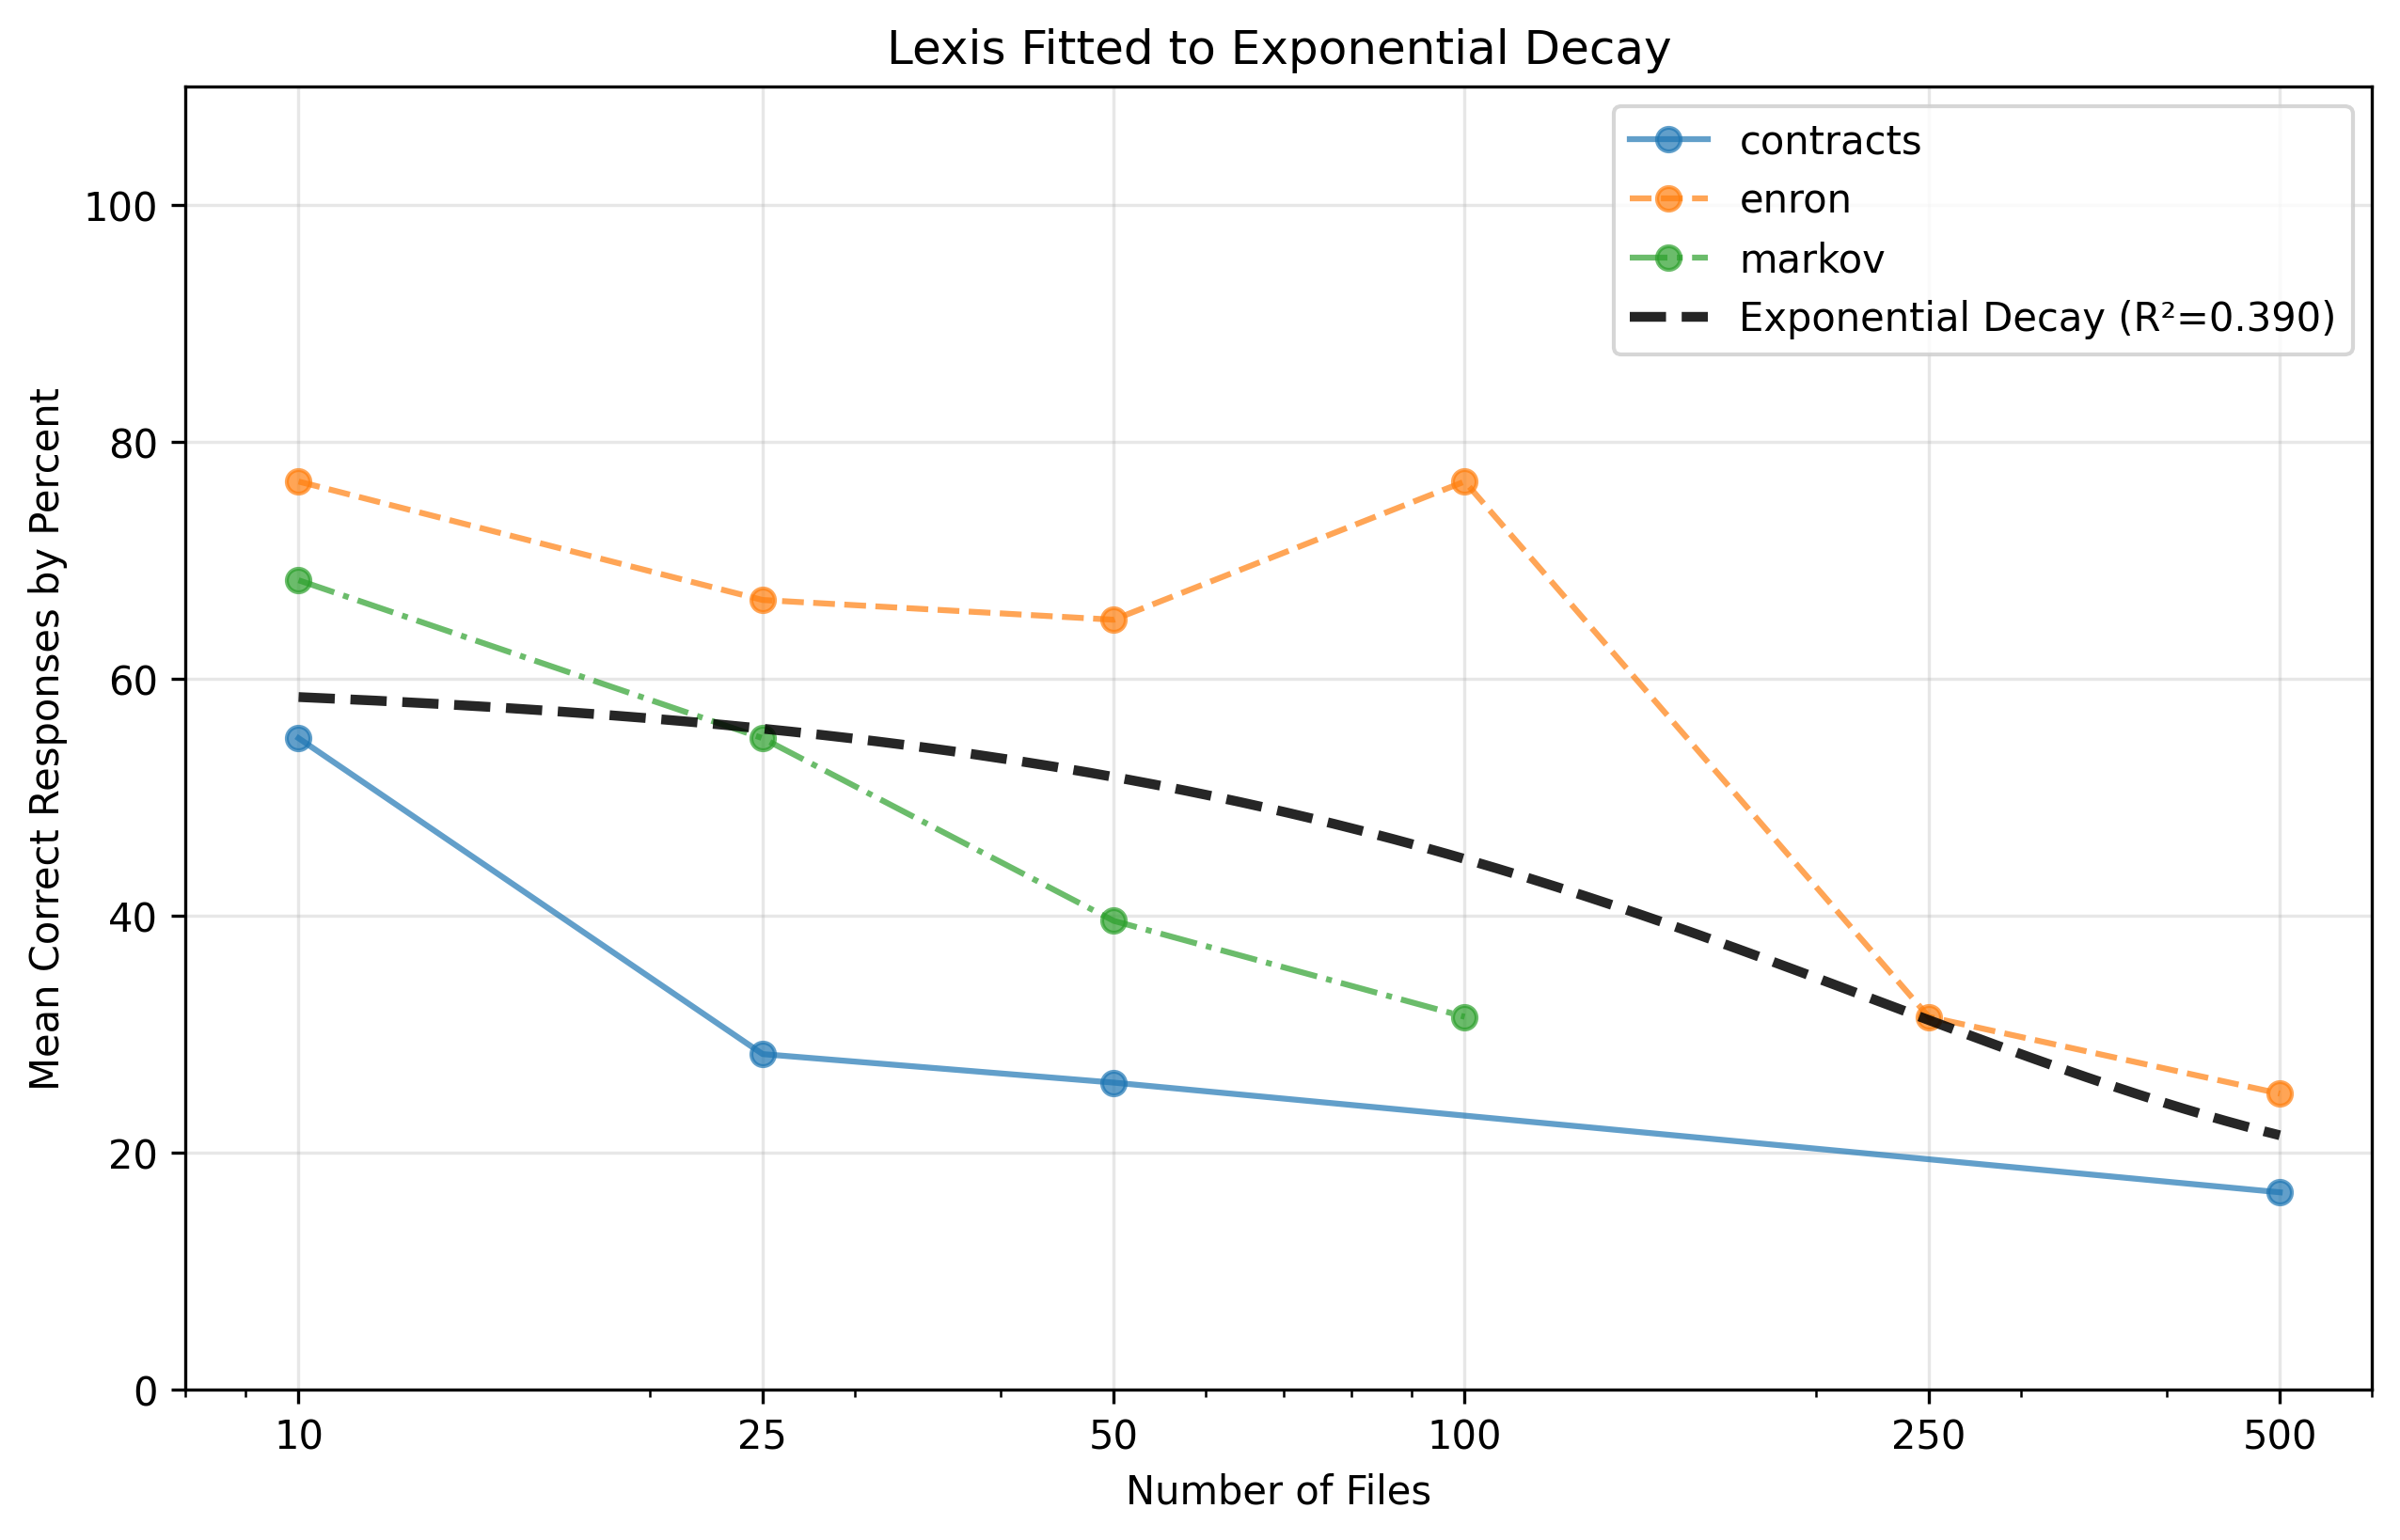
\includegraphics[width=6.25in,height=\textheight,keepaspectratio,alt={Figure 1: Lexis Performance Means by Corp}]{../data_visualizations/vendor_means/Lexis_mean_by_corp.png}

Caption: A line graph showing the performance of the Lexis Protégé
platform on retrieval performance. Each line represents a different
corpus. A separate line showing a fitted exponential decay function is
overlaid.

Figure 2: Westlaw Means by Corp
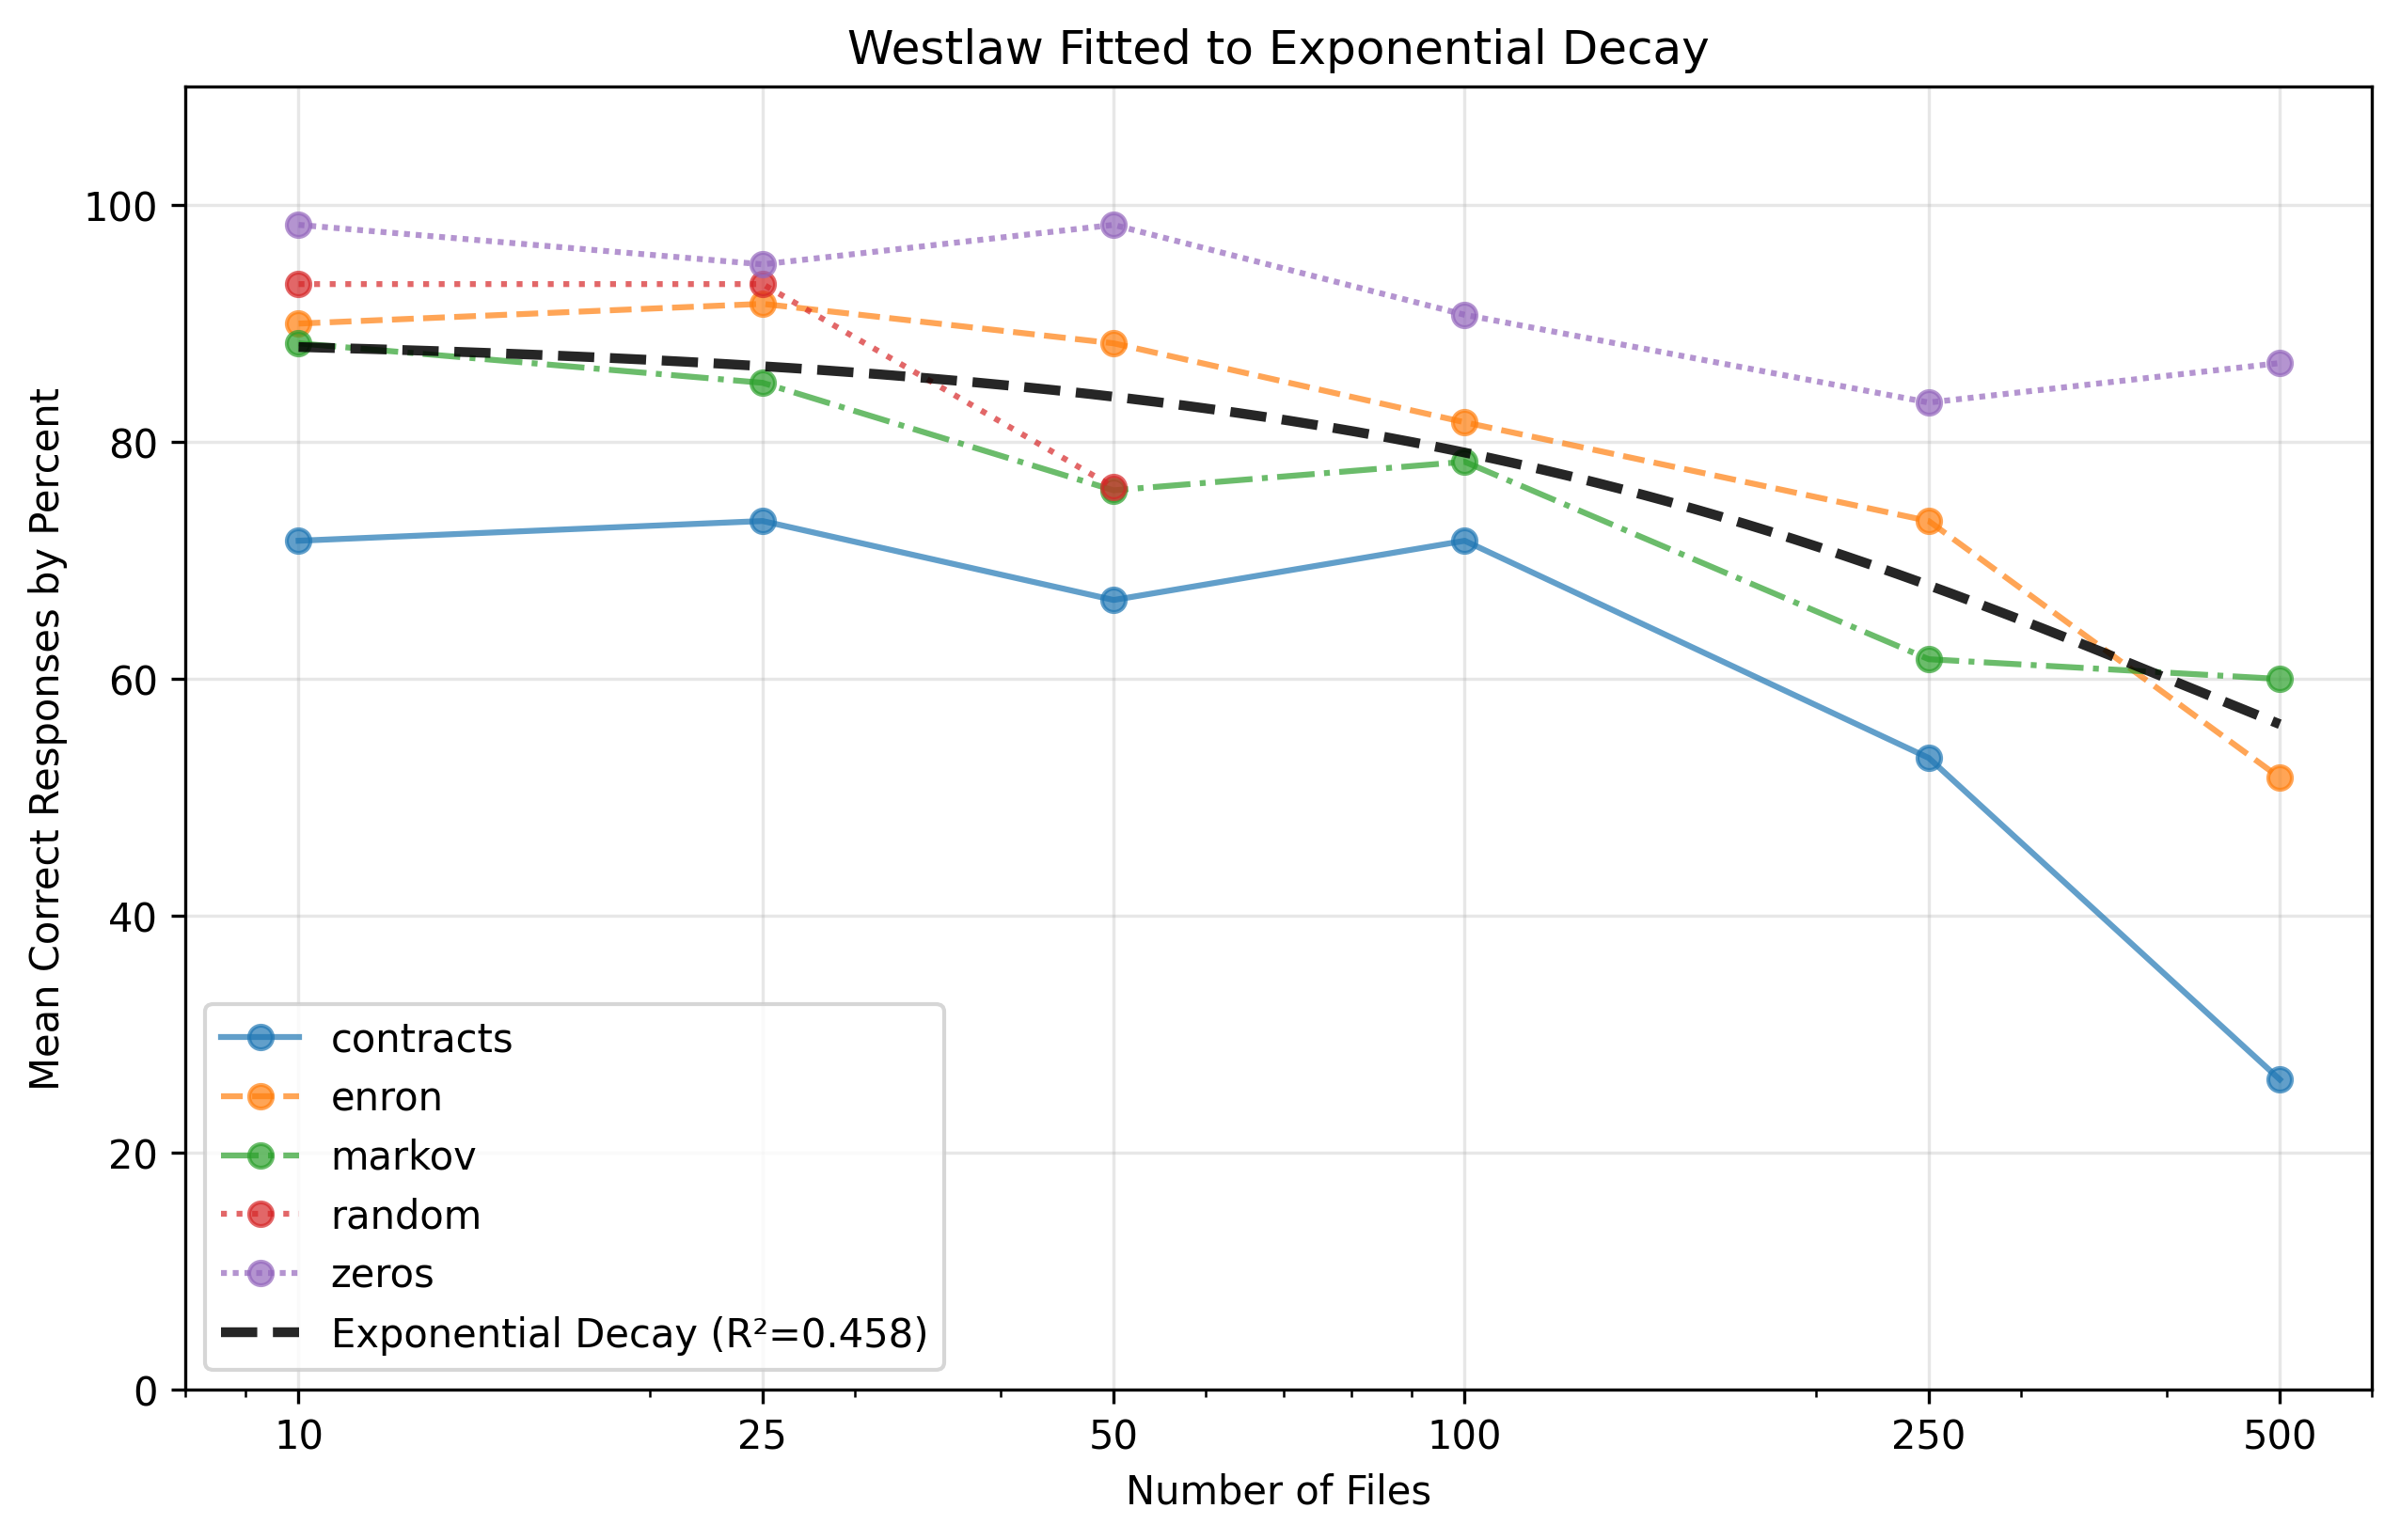
\includegraphics[width=6.25in,height=\textheight,keepaspectratio,alt={Figure 2: Westlaw Means by Corp}]{../data_visualizations/vendor_means/Westlaw_mean_by_corp.png}

Caption: A line graph showing the performance of the Westlaw CoCounsel
platform on retrieval performance. Each line represents a different
corpus. A separate line showing a fitted exponential decay function is
overlaid.

As a goodness-of-fit measure, the \(R^2\) of Lexis (0.506) and Westlaw
(0.442) shows that the exponential decay function meaningfully describes
a trend in the data, explaining \textasciitilde51\% and
\textasciitilde44\% of the variance in the data respectively. While the
exponential decay function is descriptive of the collected data, there
is also variability in the data. This \(R^2\) is influenced by a number
of factors. Because file set sizes scale approximately logarithmically,
gaps between file set sizes (x-values) are likewise spaced
logarithmically. These increasing gaps between recorded x-values can
make function fitting a challenge. Despite this challenge, exponential
decay is still clearly observable and describable within the x-value
range.

Additionally, this function is fit to data averaged from all corpora for
each given file set size. In reality, it is likely that there are
different parameters for different corpora, and that modeling a function
on each corpus individually either with custom parameters
(\(y = a_{corpus}e^{-b_{corpus}x} + c_{corpus}\)) or adding a delta
offset for each corpus (\(y = ae^{-bx} + c + \delta_{corpus}\)) would
yield a higher \(R^2\) value. While this is an interesting area for
further research, this would likely require much more data-gathering and
is outside the scope of this study to record data at a volume that is
statistically significant.

Although the primary focus of this model fitting is descriptive and not
predictive, Mean Absolute Error (MAE) describes the average amount that
predictions made on the basis of this model would be off by.
Interpretively, the given amounts show that in general, MAE shows that
Westlaw's responses generally showed less variation in its mean
responses, whereas Lexis's responses had more mean variation.

Note that due to its errors and refusals, the curve describing Lexis'
performance was fit on less data from Lexis than the other legal AI
tools.

\subsubsection{Harvey}\label{harvey}

Figure 3: Harvey Performance Means by Corp
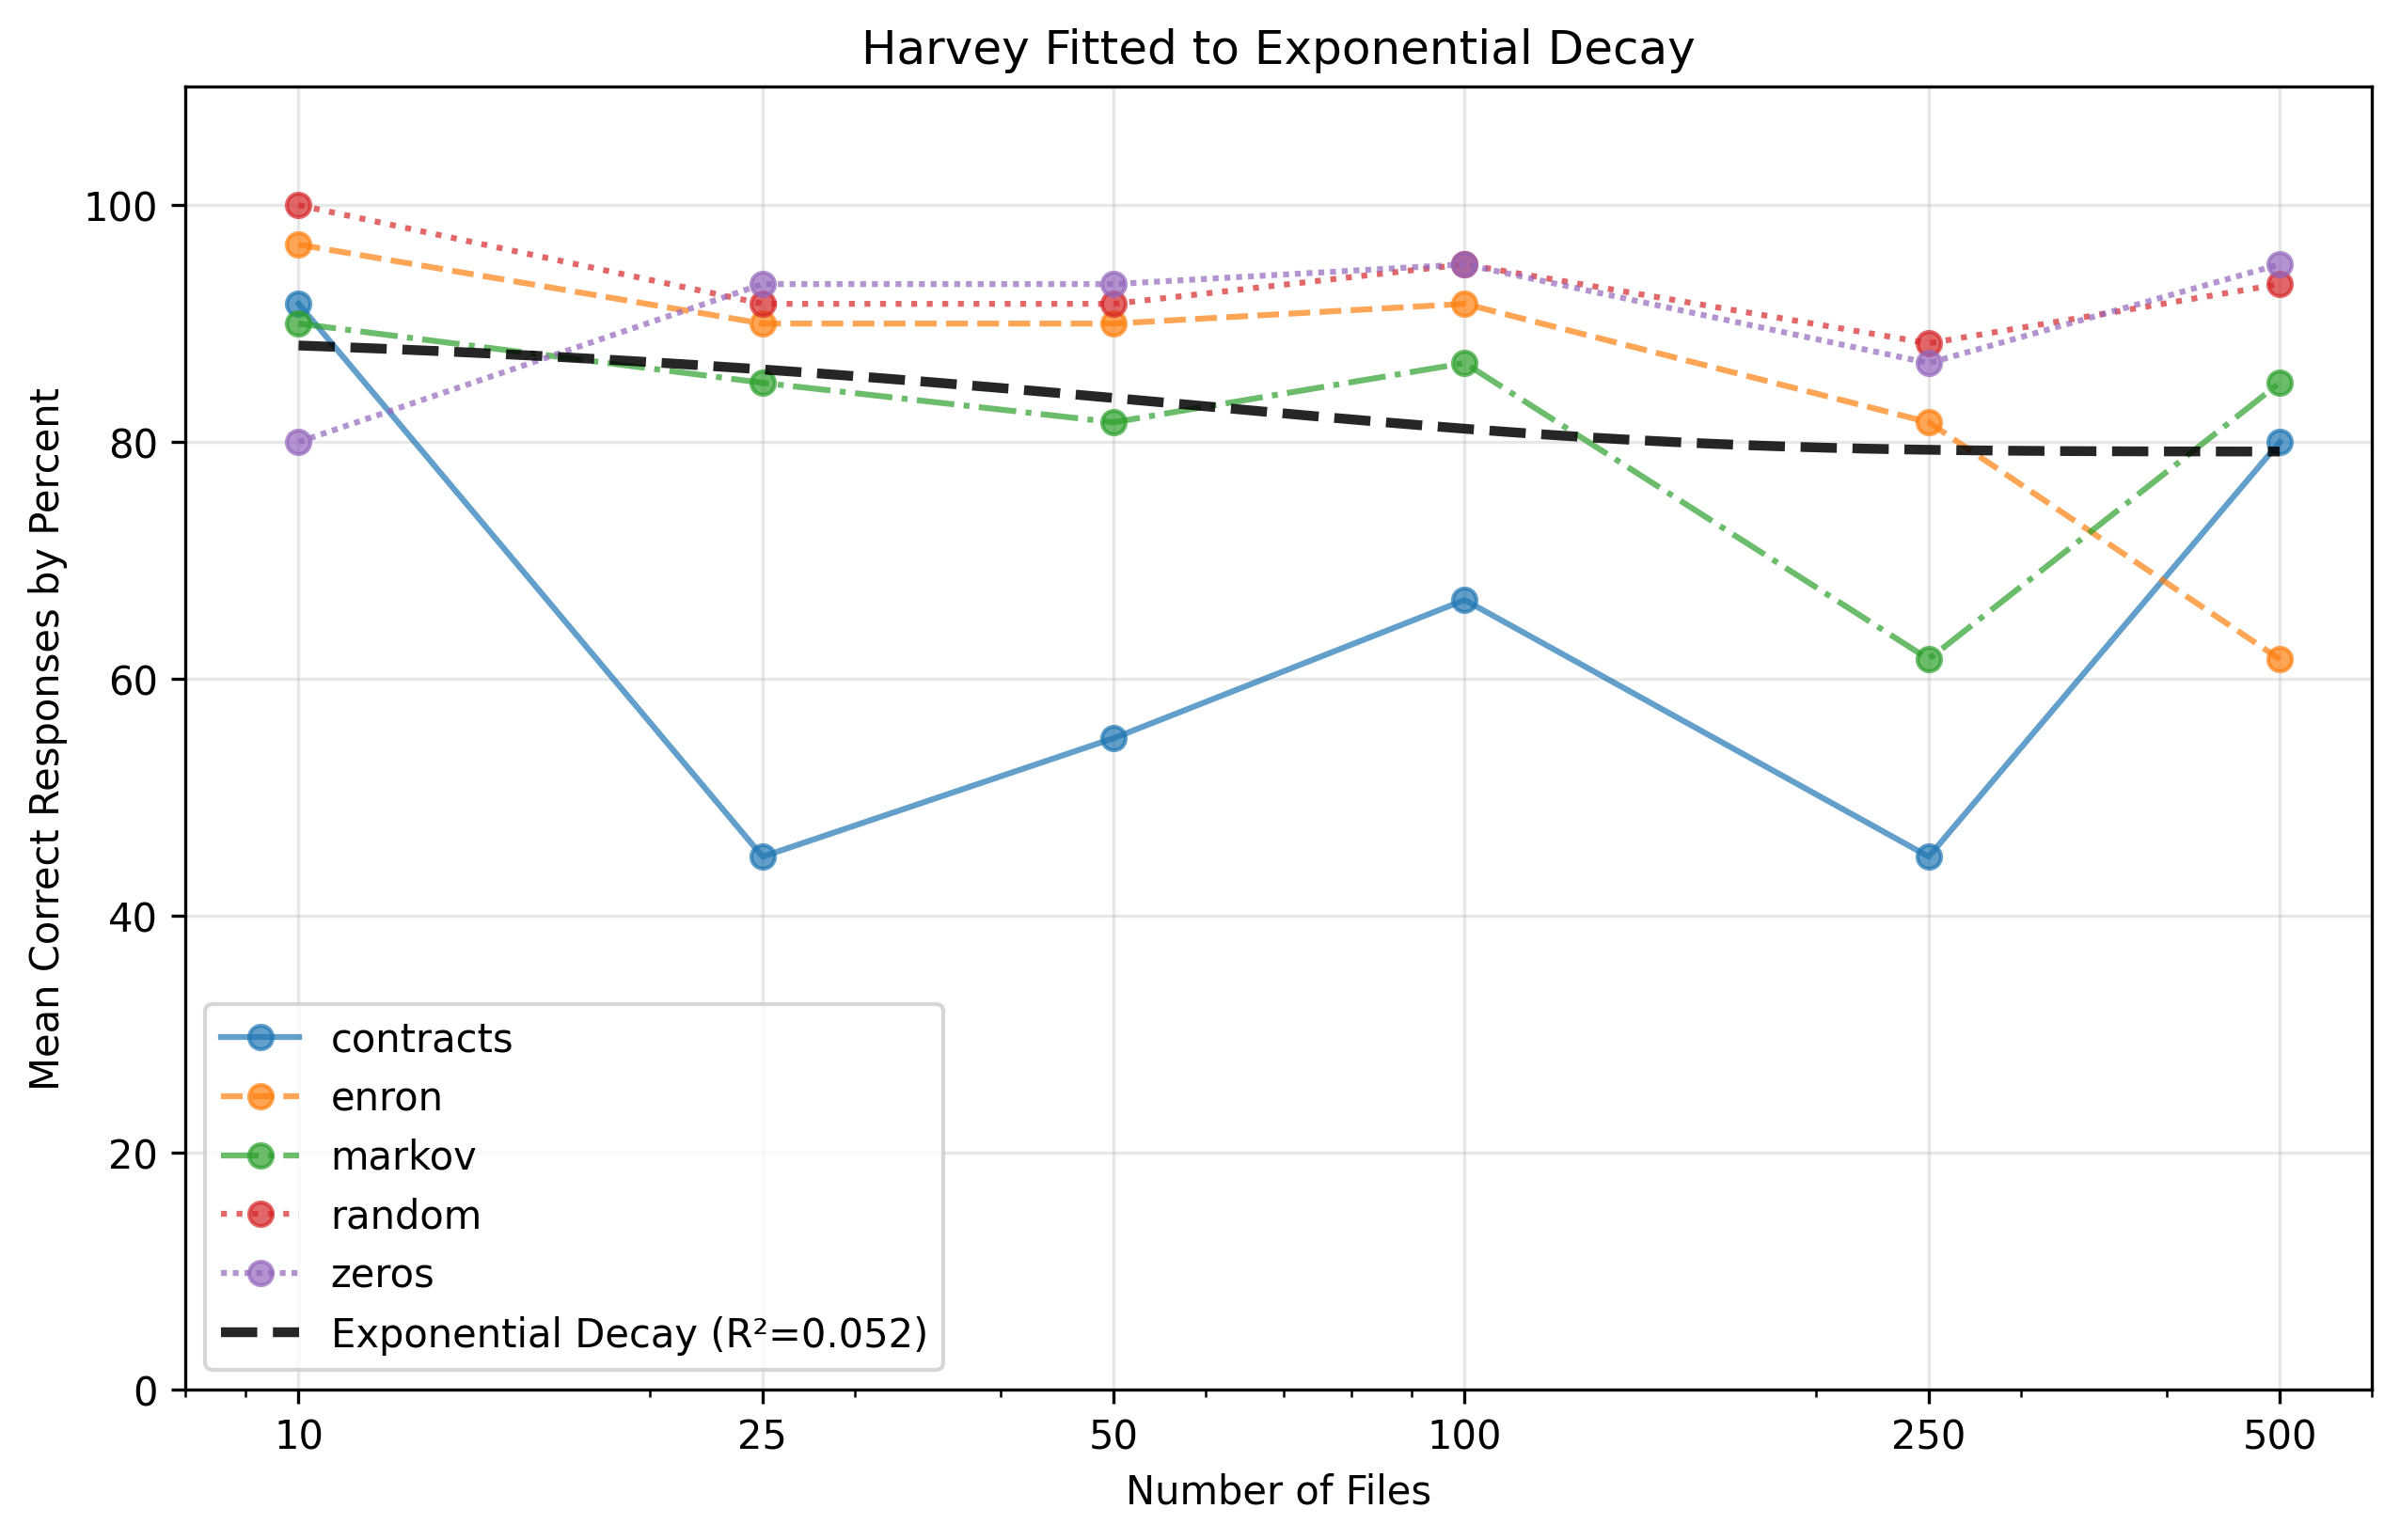
\includegraphics[width=6.25in,height=\textheight,keepaspectratio,alt={Figure 3: Harvey Performance Means by Corp}]{../data_visualizations/vendor_means/Harvey_mean_by_corp.png}
Caption: A line graph showing the performance of the Harvey platform on
retrieval performance. Each line represents a different corpus. A
separate line showing a fitted exponential decay function is overlaid,
although its poor fit is noted.

Unlike Lexis and Westlaw which fit to a exponential decay function with
statistically representative R-Values, data exploration found that no
function properly fit the data from Harvey. The line shown in the graph
shows the best-fitting exponential decay curve, but it fits the data
very poorly (\(R^2 = 0.051\)), and looks very linear. This line is
visually included to show what may be an averaged overall trend, not to
indicate fit. There is no real relationship between the fit set size and
performance that fit a regression model.

In lieu of an appropriately representative model, this study instead can
only describe Harvey's performance across all file set sizes as
centering around 83.3\% ± 10\% when all corpora are averaged (range:
73.3\% - 91.7\%).

\subsection{Correlation between Corpora and Legal AI
Performance}\label{correlation-between-corpora-and-legal-ai-performance}

There is correlation between the corpora and the Legal AI performance.

I performed Analysis of Variance (ANOVA) on all data points for each
corpora to determine whether performance of different corpora are
statistically distinct. ANOVA asks whether, for a given set of data
containing labels and values, the variation within each label is greater
than the variation between the labels. Stated differently, ANOVA
determines whether the variance between groups was greater than
variation within groups. The null hypothesis for ANOVA is that was that
performance for every corpus was the same:

\(H0: contracts = enron = markov = random = zeros\)

and the alternative hypothesis stated as:

\(Halt\): it is not the case that
\(contracts = enron = markov = random = zeros\)

The task of ANOVA is to calculate a P-value, which is a mathematical
representation of the comparison the variation within groups vs between
groups. If the P-value is lower than a selected significance level, then
we reject the null hypothesis and accept its negation, the alternative
hypothesis.

In this case, ANOVA yielded a P-value of 3.2642672702541746e-46, far
smaller than any conventional significance level. This means there is
extremely strong evidence that at one or several groups differ from
other groups.

I followed this with a variation of Tukey's Honestly Significantly
Different test called Tukey-Kramer. Tukey tests can be used when the
null hypothesis in ANOVA is rejected. It performs a similar comparison,
but between each individual pair of labels as opposed to considering
labels as a whole. The Tukey-Kramer variation is used when different
data labels had different numbers of data points. This test determines
which pairs of groups were statistically distinct from each other.

Tukey-Kramer yielded the following analysis for each pair of corpora
compared against a 5\% significance value:

{\def\LTcaptype{none} % do not increment counter
\begin{longtable}[]{@{}llrrc@{}}
\toprule\noalign{}
Group 1 & Group 2 & dij & HSD & Reject? \\
\midrule\noalign{}
\endhead
\bottomrule\noalign{}
\endlastfoot
contracts & enron & 1.1907 & 0.40118 & True \\
contracts & markov & 0.90326 & 0.41037 & True \\
contracts & random & 2.2610 & 0.49120 & True \\
contracts & zeros & 2.2227 & 0.44637 & True \\
enron & markov & 0.28742 & 0.39923 & False \\
enron & random & 1.0703 & 0.48193 & True \\
enron & zeros & 1.0321 & 0.43615 & True \\
markov & random & 1.3577 & 0.48960 & True \\
markov & zeros & 1.3195 & 0.44462 & True \\
random & zeros & 0.038250 & 0.52015 & False \\
\end{longtable}
}

For each pair of groups, the null hypothesis in Tukey-Kramer is:

\(H_{0}\) = \(group 1 = group 2\),

and the alternative hypothesis is

\(H_{alt}\) = It is not the case that \(group1 = group2\).

The ``Reject?'' column describes whether on the basis of the
Tukey-Kramer methodology, the null hypothesis is rejected and the
alternative hypothesis is adopted. Here, the alternative hypothesis is
adopted for all pairs except Enron with Markov, and Random with Zeros.
This means that according to Tukey-Kramer, the variation within each
group in a pair does not exceed the variation between the groups in
these pairs. For all other groups, the distinction is statistically
significant.

Figure 4: Performance by Corpora
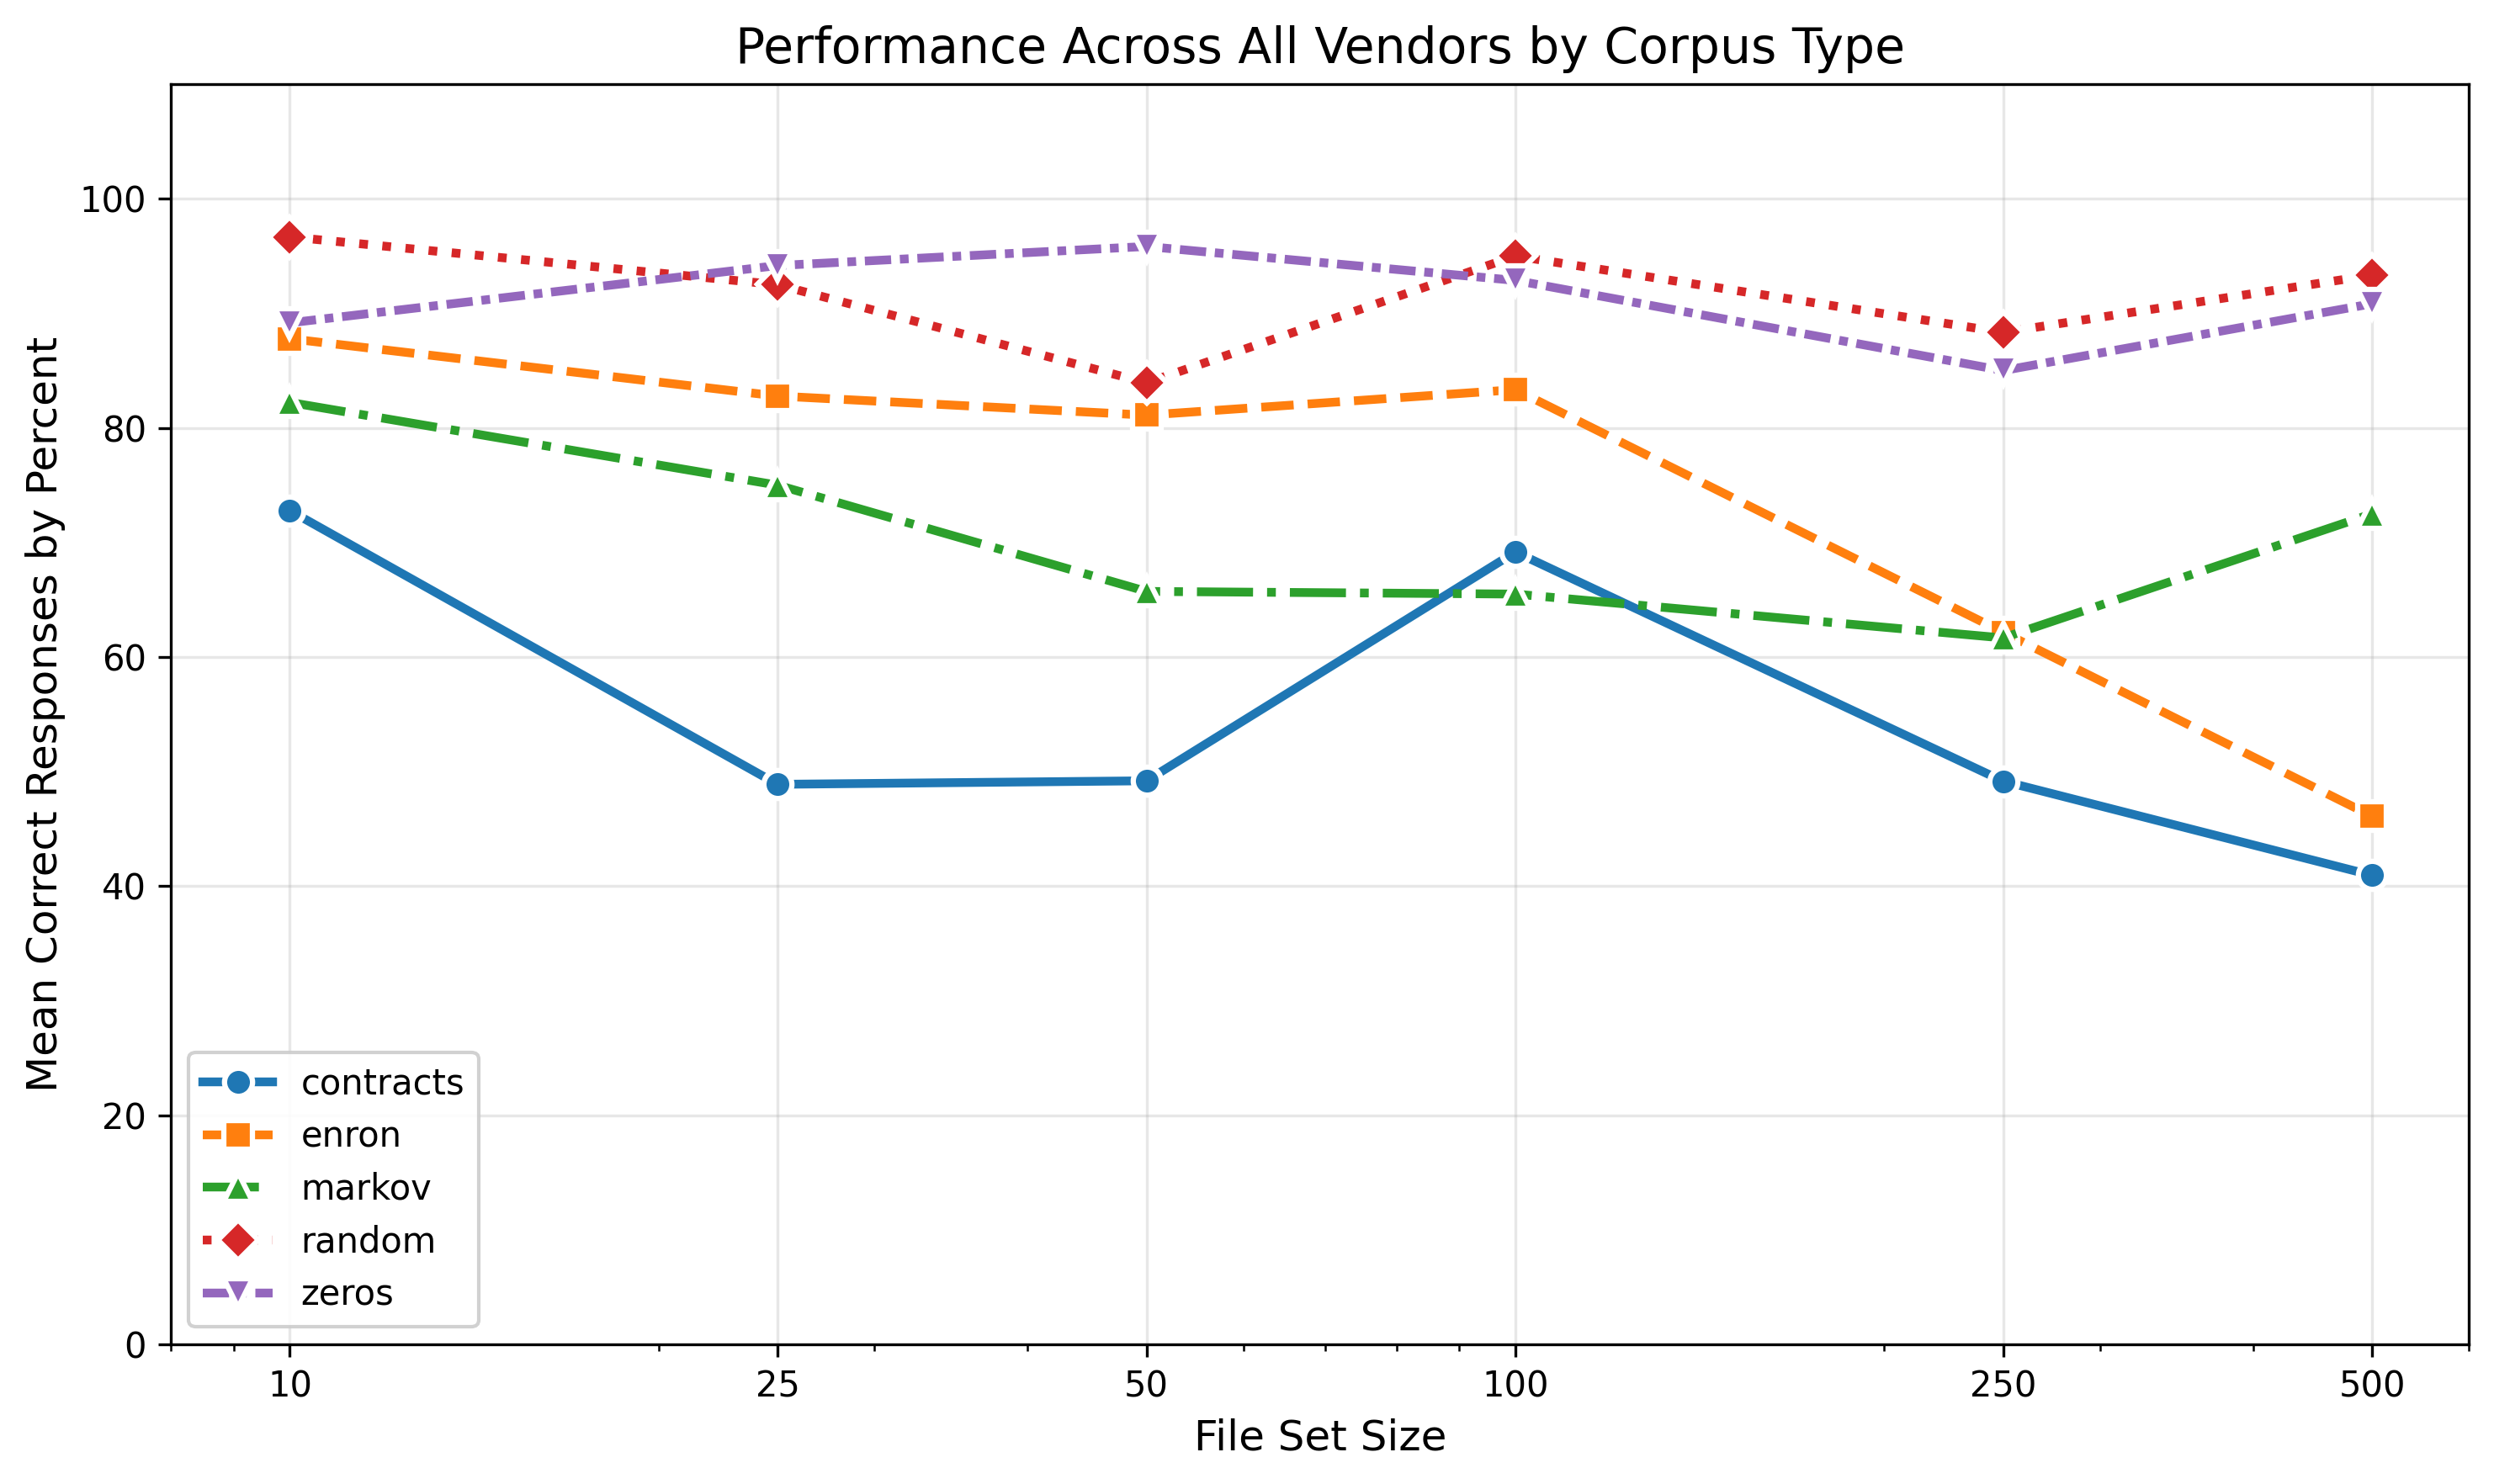
\includegraphics[width=6.25in,height=\textheight,keepaspectratio,alt={Figure 4: Performance by Corpora}]{../data_visualizations/corpora_compared/corpus_comparison.png}

After determining that there is statistical difference overall as well
as most pairs of groups, I compare these differences. The best recorded
performances came from Zeros and Random. Although note that this data
may be skewed because data is missing from Lexis for these corpora.
After Zeros and Random, the next corpora, in order of performance, is
Enron, then Markov, followed by Contracts.

The least performant corpus was Contracts. This result is surprising
because analysis of large volumes of contracts is sometimes an
explicitly advertised use of these legal AI tools. The poor performance
may be due to the density of information in the original underlying
corpus. Perhaps because of the high volume and density of legally
significant semantic content in the underlying data, all legal AI tools
seemed to suffer significantly in terms of performance. At nearly every
file size, nearly all vendors performed the worst with the Contracts
corpora.

This may indicate an inherent challenge for retrieval based legal AI
tools. Retrieval architectures pair a set of documents with a large
language model which can use it as a basis of knowledge that is outside
of its context window and outside of the information represented in its
training corpus. Retrieval architectures such as Retrieval Augmented
Generation is widely used in many legal AI architectures to increase
accuracy\footnote{see e.g.~James Ju, \emph{Retrieval-augmented
  generation in legal tech}, \textsc{Thomson Reuters Blog} (December 4,
  2024),
  https://legal.thomsonreuters.com/blog/retrieval-augmented-generation-in-legal-tech/
  {[}https://perma.cc/CM78-KFSB{]}.}, sometimes even leading to claims
that such such systems enable a legal AI to generate a response that is
``hallucation free''\footnote{LexisNexis, \emph{LexisNexis Launches
  Lexis+ AI, a Generative AI Solution with Hallucination-Free Linked
  Legal Citations}, \textsc{LexisNexis News} (October 25, 2023),
  https://www.lexisnexis.com/community/pressroom/b/news/posts/lexisnexis-launches-lexis-ai-a-generative-ai-solution-with-hallucination-free-linked-legal-citations
  {[}https://perma.cc/D24V-JADS{]}}. Such claims have been\footnote{see
  e.g.~Varun Magesh et al., \emph{Hallucination-Free? Assessing the
  Reliability of Leading AI Legal Research Tools}, \textsc{J. Empirical
  Legal Stud.} 1--27 (2025),
  https://dho.stanford.edu/wp-content/uploads/Legal\_RAG\_Hallucinations.pdf}
and should be critically examined.

The order of legal AI performance by corpora, interestingly, seems to
follow roughly the expected performance that a human would have if
presented with the same tasks. Clues among corpora that are easy to
dismiss as meaningless (Zeros and Random) had the best results, and
information containing more cognizable and semantically meaningful
information yielded worse performance.

\section{Discussion and Other
Findings}\label{discussion-and-other-findings}

The following observations are derived from extensive interaction with
the studied legal AI platforms and provide context for
statistically-determined quantitative findings.

\subsection{Platform Speed}\label{platform-speed}

The speed of these legal AI tools varies widely at each stage. For
reasons mostly unknown, Lexis was, by far, the slowest to upload files.
The only information I received that may contribute to explaining why
came from Lexis themselves. During my experimentation, a Lexis employee
contacted me and informed me that my use load was negatively impacting
``the product's overall performance''\footnote{Email from Adriana
  Ramirez, Research Attorney Practice Area Consultant, to Justin Tung,
  Reference Librarian and Lecturer at the Univ. Tex., (Feb 4, 2026 7:46
  AM CST) (on file with author).}. They explained that this was leading
to slower upload and processing times. Although they did not ask me to
stop or throttle my access, they did ask about the nature of my use to
better allocate resources for it. First, this may be indicative of
overall scale issues with the this legal AI in its current deployment.
Second, this may explain the performance of Lexis' legal AI tool in this
study. Without further information, I cannot conclusively address either
issue.

Westlaw was very fast to upload files to, but running a query through
the Legal AI can be extremely slow. With large file set sizes, responses
often took upwards of 10 minutes.

Harvey's upload and query process was unparalleled in terms of speed and
ease of use. Files uploaded quickly, had minimal errors, and the query
process did not seem to take much longer on 500 files than it did on 50.

\subsection{Performance Between Problem
Types}\label{performance-between-problem-types}

One limitation of this study is that problems of different types were
not individually recorded. I made this decision in order to manage the
scope of the research, prioritizing more data that could hopefully be
more representative of a more focused set of variables rather than less
data at a higher specificity. This area is ripe for further exploration
and analysis, and could have a significant impact on the ability to
develop functional guidelines and best practices for use of legal AI
tools.

However, from informal observation, it seemed that Simple Retrieval
tasks were the easiest for all legal AI tools, and Formal Logic was the
hardest.

\subsection{Struggles With
Non-linearity}\label{struggles-with-non-linearity}

The difficulty with Formal Logic seemed to especially stem from tasks
that required non-linear retrieval. For instance, if was clue template
was:

\begin{verbatim}
"{x} and {y} do not both know of {topic}.",
"{y} knows of {topic}."
\end{verbatim}

and the corresponding question was:

\begin{verbatim}
"ques": "Does {x} know of {topic}?"
\end{verbatim}

Reaching a conclusive answer requires the legal AI to not only find and
analyze information about \{x\}, the name explicitly given in the
answer, but also \{y\}, who is not named in the answer. Many times, the
legal AI would simply respond that either \{x\} or \{y\} knows of the
topic, showing that it likely did not make that logical step in
appropriately modifying its scope to retrieve the information it used to
formulate its answer.

Like differing problem types, further research into this dynamic could
instrumentally impact the development of guidelines and best practices
for legal AI use.

\subsection{Processing Paralleliztion}\label{processing-paralleliztion}

Through interaction with the platform, I speculate that the consistency
of Harvey's performance across different file set sizes is due to
parallelization, i.e.~the use of parallel processes that simultaneously
spawn multiple instances of an LLM to ingest and process files from the
set. This is specualtion is based on the fact that Harvey's response
times seemed roughly constant across different file set sizes, whereas
other legal AI response times scaled in porportion to the file set size.
Although parallelization an extremely powerful technique, one drawback
to this architecture is that it can lead to heavy processing demands and
high computing costs. This architecture trades processing and costs for
speed.

Harvey's different technique may be a reflection of a different product
strategy than Lexis and Westlaw. Without the ability to directly control
and query an enormous database of legal materials\footnote{Harvey does
  provide a way to integrate its platform with Lexis, but this is not
  part of its base product, which is the product this study evaluated.},
Harvey's product may seek competitiveness on the basis prioritizing
access to computing resources. Because they also do not have the cost
burden of maintain such a database, they may still stay cost-competitive
even though they offer a product with different capabilities.

\section{Conclusion}\label{conclusion}

The legal tech market often seems to have an infinite amount of AI
products purporting to sell any imaginable kind of functionality.
However, the majority of available information about these tools comes
from marketing material and first-party sources. Without independent
scrutiny and analysis, it is easy to mistake anecdotal success for
statistically impactful utility.

To test the impact of the number of files and the type of content in
those files on the performance of different legal AI tools, I created
file sets of five corpus types at six file set sizes to test the custom
database retrieval capabilities of legal AI tools from Harvey, Westlaw,
and Lexis. I injected these file sets with clues and questions pulled
from a standardized template which was varied enough to avoid
cross-contamination. I then repeated ten total trials per condition, and
measured the ability of the legal AI tool to retrieve the relevant clues
required to be responsive to the question. In total, I uploaded over
140,000 files across 900 vaults.

First, to test the influence of file set size on a legal AI's
performance, I found that Westlaw's performance could be meaningfully
described with an exponential decay model, beginning with an average of
88.3\% at a file set size of 10, and ending at 54.2\% at a file set size
of 500. Lexis' performance could also be meaningfully described with an
exponential decay model, beginning with an average of 66.7\% at at file
set size of 10 and ending at 18.7\% at a file set size of 500.
Additionally, no recorded data was available for two entire corpora and
some file set sizes for another corpora. Harvey's performance did not
fit an exponential decay model, nor any other mathematical model
attempted, and instead began by accurately retrieving 91.7\% of answers
at a file set size of 10, and 83.0\% of answers at a file set size of
500. Through the range, Harvey's performance centered around 83.3\%.

Second, to test the influence of different corpora on the performance of
all legal AI, I used the ANOVA method to reject the Null Hypothesis that
there is no statistically significant difference between groups based on
their labels, then used the Tukey-Kramer test to determine in which
pairs of corpora those statistically significant differences appeared. I
found that with the exception of two pairs (Enron + Markov; Random +
Zeros), all other pairs of corpora showed distinguishable differences,
meaning that the variation between the two groups was greater than the
variation within each individual group.

These findings support the conclusion that the performance of legal AI
tools from Westlaw and Lexis decreases as the volume of user-uploaded
files increases. These findings also show that the performance of all
tested legal AI tools is influenced by the type of data in the uploaded
files, with some types of text yielding more accurate results than
others.

The practical implications of this information are manifold. Since
performance increases with smaller file set sizes, users of legal AI
products may focus on reducing the amount of uploaded information when
possible to maximize performance when using Westlaw or Lexis. There may
also be a file set size threshold with Westlaw and Lexis beyond which
their lack of accuracy means they should not be used. Similarly, users
should be wary of the way that different types of uploaded data can lead
to better or worse performance. Ironically, data with a high density of
legally probative statements tend to perform worse than data that does
not.

In light of these findings, a best practice may be to examine the type
of data to be uploaded before using a legal AI tool, or at least to
scrutinize the legal AI's output according to an awareness of that data.
Additionally, some legal AI tools also show a decay in performance as
the amount of uploaded material increases. Together, the findings of
this study supports a view of legal AI tools which have high perform
under certain conditions and low performance under others. Users of
these tools ought to determine their threshold of acceptable performance
for a given task to decide whether the legal AI tool is the correct tool
to use.

Aggregating these use cases can also inform purchasing decisions, as the
cost of the legal AI tool can be weighed against the utility of that
tool, as well as compared to competing tools on the market.

This study leaves to further research the differences in kinds of
questions such as rote retrieval and linearity. It also leaves to
further research the effect of scaling clue density with file set sizes.
Much of this research requires a larger sample size per condition in
order to draw statistically significant results, which was outside this
study's scope.

In the context of the ever-changing legal tech market, some AI tools and
their providers claim that their product will bring powerful
transformations to the practice of law. This study scrutinizes a subset
of those claims, specifically relating to the ability to upload a custom
database and query it with a legal AI tool.

\end{document}
